%Rayleigh and Mei scatteing theory mit plots
\section{Visibility}
\label{sec:visib}
Since this study focuses on forecasting visibility, the most important definitions, mathematical derivations and physical processes related to it, are presented in this Section.
\subsection{Definitions}
The World Meteorological Organization (WMO) sets all standards and definitions for meteorological measurements, forecasts and procedures, including visibility observation. It  provides three important definitions in the context of visibility \cite{WMO}:
\begin{itemize}
    \item {The \textbf{meteorological optical range} is the length of path in the atmosphere required to reduce the luminous flux in a collimated beam from an incandescent lamp, at a colour temperature of 2700 K, to 5\% of its original value, the luminous flux being evaluated by means of the photometric luminosity function of the International Commission on Illumination (CIE). }
    \item{ \textbf{Visibility, meteorological visibility (by day) and meteorological visibility at night} are defined as the greatest distance at which a black object of suitable dimensions (located on the ground) can be seen and recognized when observed against the horizon sky during daylight or could be seen and recognized during the night if the general illumination were raised to the normal daylight level.}
    \item { \textbf{Visual range (meteorological)}: Distance at which the contrast of a given object with respect to its background is just equal to the contrast threshold of an observer.}
\end{itemize}


%This thesis focuses on forecasting visibility, for which \citeauthor{clark2008prediction} \cite{clark2008prediction} state the following:
%\begin{quote}
%`Visibility represents the shortest horizontal distance %visible, considering all directions'
%\end{quote}

%The `visible distance' means the distance, for which an %object is still visible for a human observer. 
%To be able to observe an object, it has to have a contrast $C$, with respect to its background, that lies above a contrast threshold value $\varepsilon$. 
Regarding their definitions, the meteorological visibility and the visual range are closely related. The meteorological visibility is mostly relevant for human observers, denoting always the lowest value considering all horizontal directions. Although the WMO sets the meteorological optical range as the measurement standard, the meteorological visibility is the recommended approximation for human observers, since it can be understood intuitively. Because most visibility measurements are still performed by human observers, meteorological visibility is the measure for visibility in praxis.\\ \\
\citeauthor{koschmeider1924theorie} was the first one to derive a mathematical expression for visibility, using the visual range \cite{koschmeider1924theorie}.\\
Also in most models the visual range is used, because it provides a more thorough definition than the meteorological visibility and is therefore easier to be implemented, but still relates to the observed visibility. The mathematical derivation is briefly outlined in the following section according to \citeauthor{price2007advanced} \cite{price2007advanced}, who refers to the works of \citeauthor{koschmeider1924theorie} \cite{koschmeider1924theorie}.

\subsection{Mathematical Derivation of Visibility and Visual Range}

Let the contrast $C$ be defined as 
\begin{equation}
    C=\frac{ B_{b} - B_{a} }{B_{b}} \quad ,
\end{equation}
where $B_{b}$ denotes the brightness of the background and $B_{a}$ the brightness of the object,
and let the change of the brightness on an infinitesimal line segment along a horizontal line $x$ be
\begin{equation}
    \frac{dB}{dx}=- \beta_{\mathrm{tot}}B + B_{s} \quad ,
    \label{eq:fracB}
\end{equation}
where $ \beta_{\mathrm{tot}}$ denotes the total atmospheric extinction coefficient and  $B_{s}$ denotes the light that is being scattered in the line. Equation \eqref{eq:fracB} can also be applied to $B_{b}$.
Since the brightness of the background is independent of the distance, the following condition is satisfied:
\begin{equation}
    \frac{dB_{b}}{dx}=0 \quad .
\end{equation}
Then, the change of contrast along an infinitesimal line segment can be written as
\begin{equation}
    \frac{d C }{dx} = -\frac{1}{B_{b}} \frac{B_{a}} {dx}  \quad .
    \label{eq:contrastfrac}
\end{equation}
Evaluating Equation \eqref{eq:fracB} for the brightness of the background we gain the expression
\begin{equation}
    \beta_{\mathrm{tot}}B_{b}= B_{s} \quad .
    \label{eq:background}
\end{equation}
When plugging \eqref{eq:background} into Equation \eqref{eq:fracB} and evaluating Equation \eqref{eq:contrastfrac} we get
\begin{equation}
    \frac{d C}{d x} = - \beta_{\mathrm{tot}} C
    \label{eq:CDE} \quad .
\end{equation}
As Equation \eqref{eq:CDE} implies, we can use an exponential ansatz and get the necessary boundary conditions by investigation of the case of a perfectly black object in front of a white background. In the considered scenario, the contrast of the object at the point of the observer has to be 100\%, because all light is absorbed. Also, the contrast should go to 0 for the object being infinitely far away. Hence, the following equations need to be satisfied:

\begin{eqnarray}
     C(x=0)&=&1\\
     \lim_{x \to \infty} C(x)&=&0 
\end{eqnarray}

With these boundary conditions the coefficients of the contrast are derived as an exponential function of the distance between the observer and the object
\begin{equation}
    C(x)=\exp (-\beta_{\mathrm{tot}}x) \quad .
\end{equation}
From this we can derive the maximum distance for which the contrast is still above the contrast threshold value. This distance is called the `visual range'. Since the atmospheric extinction can vary for different directions, the visual range can vary too. The minimum of the visual range, considering all directions, is approximately the visibility $vis$. For reasons of computational simplicity, we only use the atmospheric extinction of the point where the visibility is forecast. Hence, the visual range and the visibility are equivalent in this study and defined by 
\begin{equation}
    vis = -\frac{ \ln ( \varepsilon)} { \beta_{\mathrm{tot}}}    \quad .
    \label{visibility}
\end{equation}
The contrast threshold $\varepsilon$ should be chosen under the consideration of the purpose and usage of the visibility data.
Most authors suggest to set the contrast threshold to $2 \% $ (e.g. \citeauthor{ballard1992diagnosis} \cite{ballard1992diagnosis}) while other consider  $5 \% $ to be more accurate  (e.g. \citeauthor{claxton2008using} \cite{claxton2008using}). 
The differing values are due to the fact that the contrast is chosen with respect to what our eyes are gauged to. But as we experience in our everyday life, this can vary for different people, shapes and colours \parencite{koschmeider1924theorie}. As this implies, the constant setting of $\varepsilon$ is an approximation for the sake of simplicity. 






\subsection{Atmospheric Scattering}


Mie and Rayleigh scattering are special cases of scattering of electromagnetic waves on a homogeneous sphere \cite{hulst1957light}. Both scattering regimes together are sufficient to describe the most important scattering processes in the atmosphere.  Mie scattering, for example, is responsible for visibility reduction due to fog and for clouds being perceived as white. To observe the effects of Rayleigh scattering, one must simply look at the  blue colour of the clear sky \cite{wallace2006atmospheric}. 
Generally, if we aim to describe a radiative process with one of the two theories, we need to verify first, if it is suitable for the process' size range. To be able to do so, a size parameter $\alpha$ is introduced. It depends on the radius of the sphere $r$ and the wavelength of the incoming light $\lambda$ and is defined as
\begin{equation}
    \alpha = \frac{ 2 \pi r }{\lambda} \quad .
\end{equation}
For Rayleigh scattering the condition
\begin{equation}
    \alpha \ll 1
    \label{eq:Rayleighcon}
\end{equation} must hold. In other words, the radius of the object must be much smaller than the wavelength of the incoming radiation.
In the Earth's atmosphere Rayleigh scattering is mostly contributed by scattering on air molecules and much less variable in time and space than the contribution by Mie scattering. \\
Another difference between the to regimes is that Rayleigh scattering strongly favours shorter wavelengths and therefore in the visible spectrum the colour blue. Mie scattering on the other hand, has a very weak dependence on the wavelength \cite{raith2001erde}. As a result we see most Mie-scattered sunlight as white, because it contains all wavelengths of the sun's spectrum.
The Mie scattering regime can be applied for all cases where 
\begin{equation}
     0.1<\alpha<50
     \label{eq:Miecondition}
\end{equation}
holds. \\
For visible light, which has a wavelength from approximately 390nm to 700nm,  the condition is satisfied for scattering on vapour, hydrometeors and aerosols \parencite{wallace2006atmospheric, chandrasekar2010basics}.
Due to the dominating physical process being Mie scattering  \parencite{price2007advanced}, there is a strong dependency of the total atmospheric extinction coefficient on the specific humidity, precipitation, cloud water in liquid and ice form and aerosols. The relations can be derived by characterizing the hydrometeors and aerosols in the air as a suspension of perfect spheres with different refractive indices and radii in a gas \cite{lang2010interaction}. Figure \ref{fig:red-on-raindrop} illustrates an example of atmospheric scattering: visible red light on a water drop. The plot shows a peak for forward scattering, typical for the angular intensity distribution of Mie scattering.
%The extinction efficiency for the different spheres is calculated and used to derive mass
\begin{figure}
    \centering
    \begin{subfigure}{0.45\textwidth}
 %       \captionsetup{width=\textwidth}
        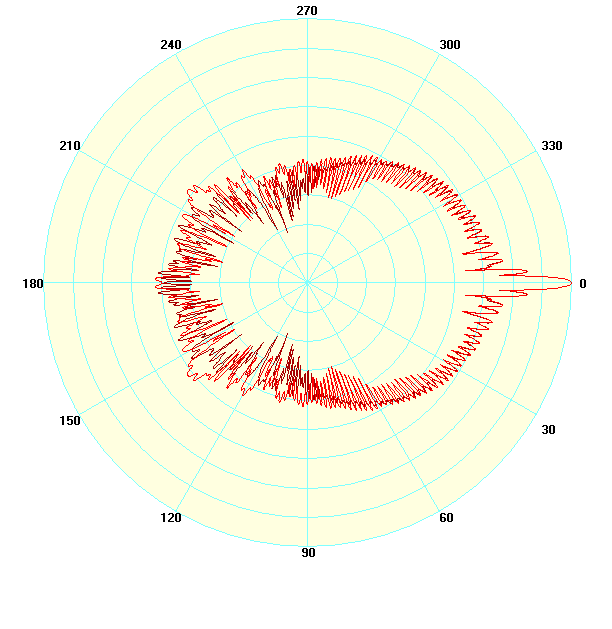
\includegraphics[width=\textwidth]{graphics/650nmonWaterEdited.png}
        \caption[Scattering on a Rain Drop]{Scattering of visible red light ($\lambda$=650nm) on a water drop.\\ Used parameters: particle radius: 1.0e-05 m; refractive index: 1.33257 + i1.67e-08; scale: logarithmic, value at outer circle: 2.18e+07, value at inner circle: 2.18e-02.\label{fig:red-on-raindrop}  }    
    \end{subfigure}
    \hspace{1cm}
    \begin{subfigure}{0.45\textwidth}
        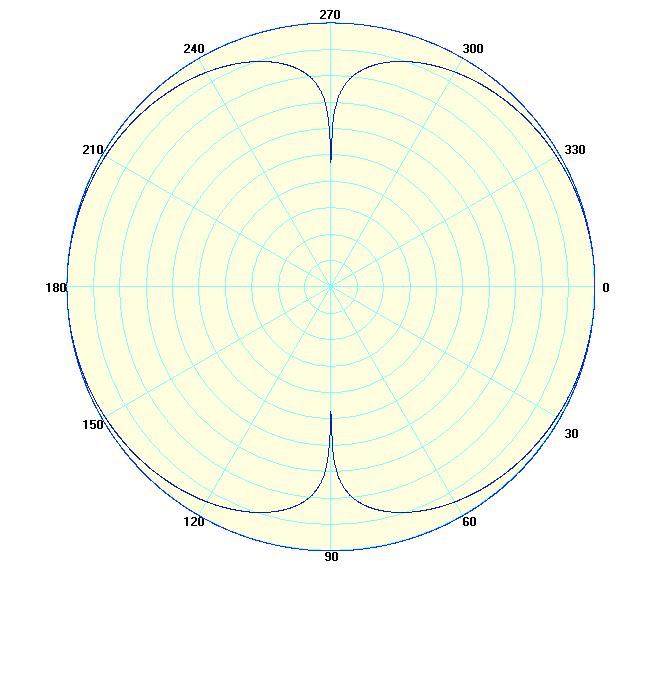
\includegraphics[width=\textwidth]{graphics/Rayleighscatter.png}
        \caption[Scattering on a Rain Drop]{Scattering of visible blue light ($\lambda$=400nm) on an oxygen molecule.\\ Used parameters: particle radius: 1.52e-10 m; refractive index: 1.000152; scale: logarithmic, value at outer circle: 2.5e-24, value at inner circle: 2.18e-34. \label{fig:blue-on-oxygen}  }
    \end{subfigure}
    \caption[Scatter Plots of Mie and Rayleigh scattering]{Scatter plot of Mie and Rayleigh scattering: Intensity versus scattering angel. \\Created by the use of \citetitle{laven2011mieplot} }
\end{figure}
%But because these quantities all interact with other model variables in a non-linear way, implicitly temperature, pressure and many other variables have great impact on the visibility as well. \\





The scattering characteristics of a material are described by their extinction, scattering and absorption coefficients. In the course of predicting  visibility, we are only interested in the extinction coefficient to be able to quantify the total reduction the light's intensity \cite{horvath1981atmospheric}.
The extinction coefficient $ Q_{ext}$ is the dimensionless equivalent of the extinction cross section $C_{ext}$ and defined as
\begin{equation}
    Q_{ext}=\frac{C_{ext}}{G} \quad ,
\end{equation}
where $G$ is the geometric factor that is set to $\pi r^{2}$ for spherical particles, because of their circular cross section.

The extinction cross section is a measure for the total difference in radiant flux through a defined surface $S$. The two compared cases are, when a particle is present at a location and when it is not. The extinction cross section is defined as 
\begin{equation}
C_{ext}=\frac{1}{E^{i}} \int_{4\pi R^{2}} (E^{i}-E)dS \quad ,
\label{eq:extcoef1}
\end{equation}
where $E^{i}$ denotes the electric field vector when there is no particle at the location, and $E$ when a particle is present. The boundary surface $S$ is set to the surface of a sphere because we are interested in the case of scattering on spherically approximated particles.
For aerosol scattering the electric field vectors can be obtained by the use of Mie scattering theory. The theory was first developed by Gustav    \citeauthor{mie1908beitrage} \cite{mie1908beitrage} and is derived by applying boundary and continuity conditions for light approaching a sphere to Maxwell's equations.\\
The resulting wave functions are in form of power series composed of Bessel functions and Legendre polynomials \parencite{kerker2016scattering}.
When inserting these in Equation \eqref{eq:extcoef1} we derive the following mathematical expression for the extinction cross section:
\begin{equation}
C_{ext}=-\frac{2 \pi }{k^{2}_{0}} \Re \left( \sum_{n=1}^{ \infty} (2n +1) (a^{s}_{n} + b^{s}_{n}) \right) \quad ,
\label{eq:extcoef2}
\end{equation}
where $k_{0}$ is the wave number in vacuum and $a^{s}_{n}$ and  $b^{s}_{n}$ are the Mie coefficients. Those are derived as part of the solution when solving the scalar wave equation. The Mie coefficients are composed of Riccati-Bessel functions and include a dependency on the refractive index. The entire detailed derivation is presented in several textbooks e.g. \cite{zdunkowski2007radiation}, \cite{hulst1957light}.
Regarding Equation \eqref{eq:extcoef2}, we see that only an approximation of $C_{ext}$ can be calculated numerically and the accuracy depends mainly on the number of terms computed. Many different algorithms for the computations were developed and \citeauthor{wriedt2009light} \cite{wriedt2009light} provides a good overview with special focus on the application on aerosols. \\
As mentioned, the second most relevant scattering process in the atmosphere is Rayleigh scattering. Regarding the criterion presented in Equation \eqref{eq:Rayleighcon}, it is obvious that Rayleigh scattering takes place, if the size of the particle is much smaller than the incoming wavelength. It is a result of the polarizability of the gas molecules: the incoming electromagnetic wave excites the molecules, so that each molecule acts as Hertzian dipole. Figure \ref{fig:blue-on-oxygen} illustrates an example of visible blue light being scattered on an oxygen molecule and shows the characteristic angular intensity distribution of a Hertzian dipole. It radiates  with the same wavelength as the incoming light. This is also true for Mie scattering.
Such processes, without a shift between the wavelength of the scattered light and the incident light, are called elastic, because the change in energy of the photons is negligibly small.
